\section{Approach}

In general, a data mining task will have the following steps - data collection, data integration and cleaning, transformation and selection, data mining and evaluation \cite{Fayyad:1996:DMK:257938.257942}. It has been estimated that data preparation - integration, cleaning, selection and transformation, accounts for a significant portion of the time spent on a data mining project. In our approach to demonstrate the end-to-end process of data preparation and data mining, we select the task of predicting the mode of transport for a user, given the sensor data collected by the mobile phones. Our approach enables users to integrate data from a variety of sources without exposing them to the underlying complexity of data integration and exchange. Figure \ref{fig:system_diagram} shows the different blocks of system.
 
\subsection{Data Collection}
We collect the mobile sensor data using a custom Android application built using the funf\footnote{http://inabox.funf.org} sensing framework. The application records the readings from the Accelerometer and the Global Positioning System (GPS) sensors, archives and uploads the collected data to a Dropbox\footnote{http://dropbox.com} account every 24 hours. Our users collected data for three days, yielding datasets consisting of Comma Separated Value (CSV) files. Each dataset is comprised of 3 files:

\begin{enumerate}
  \item \textit{LocationProbe.csv}: Contains positioning data from the GPS sensors and has 47 columns describing the user's location, speed, bearing, etc.
  \item \textit{AccelerometerSensor.csv}: Contains coordinate values from the accelerometers
  \item \textit{TransportationLabels.csv}: The user collecting the data has to label each mode of transport that they use and the specific intervals of the day when they use it
\end{enumerate} 

\begin{figure}[h]
\centering
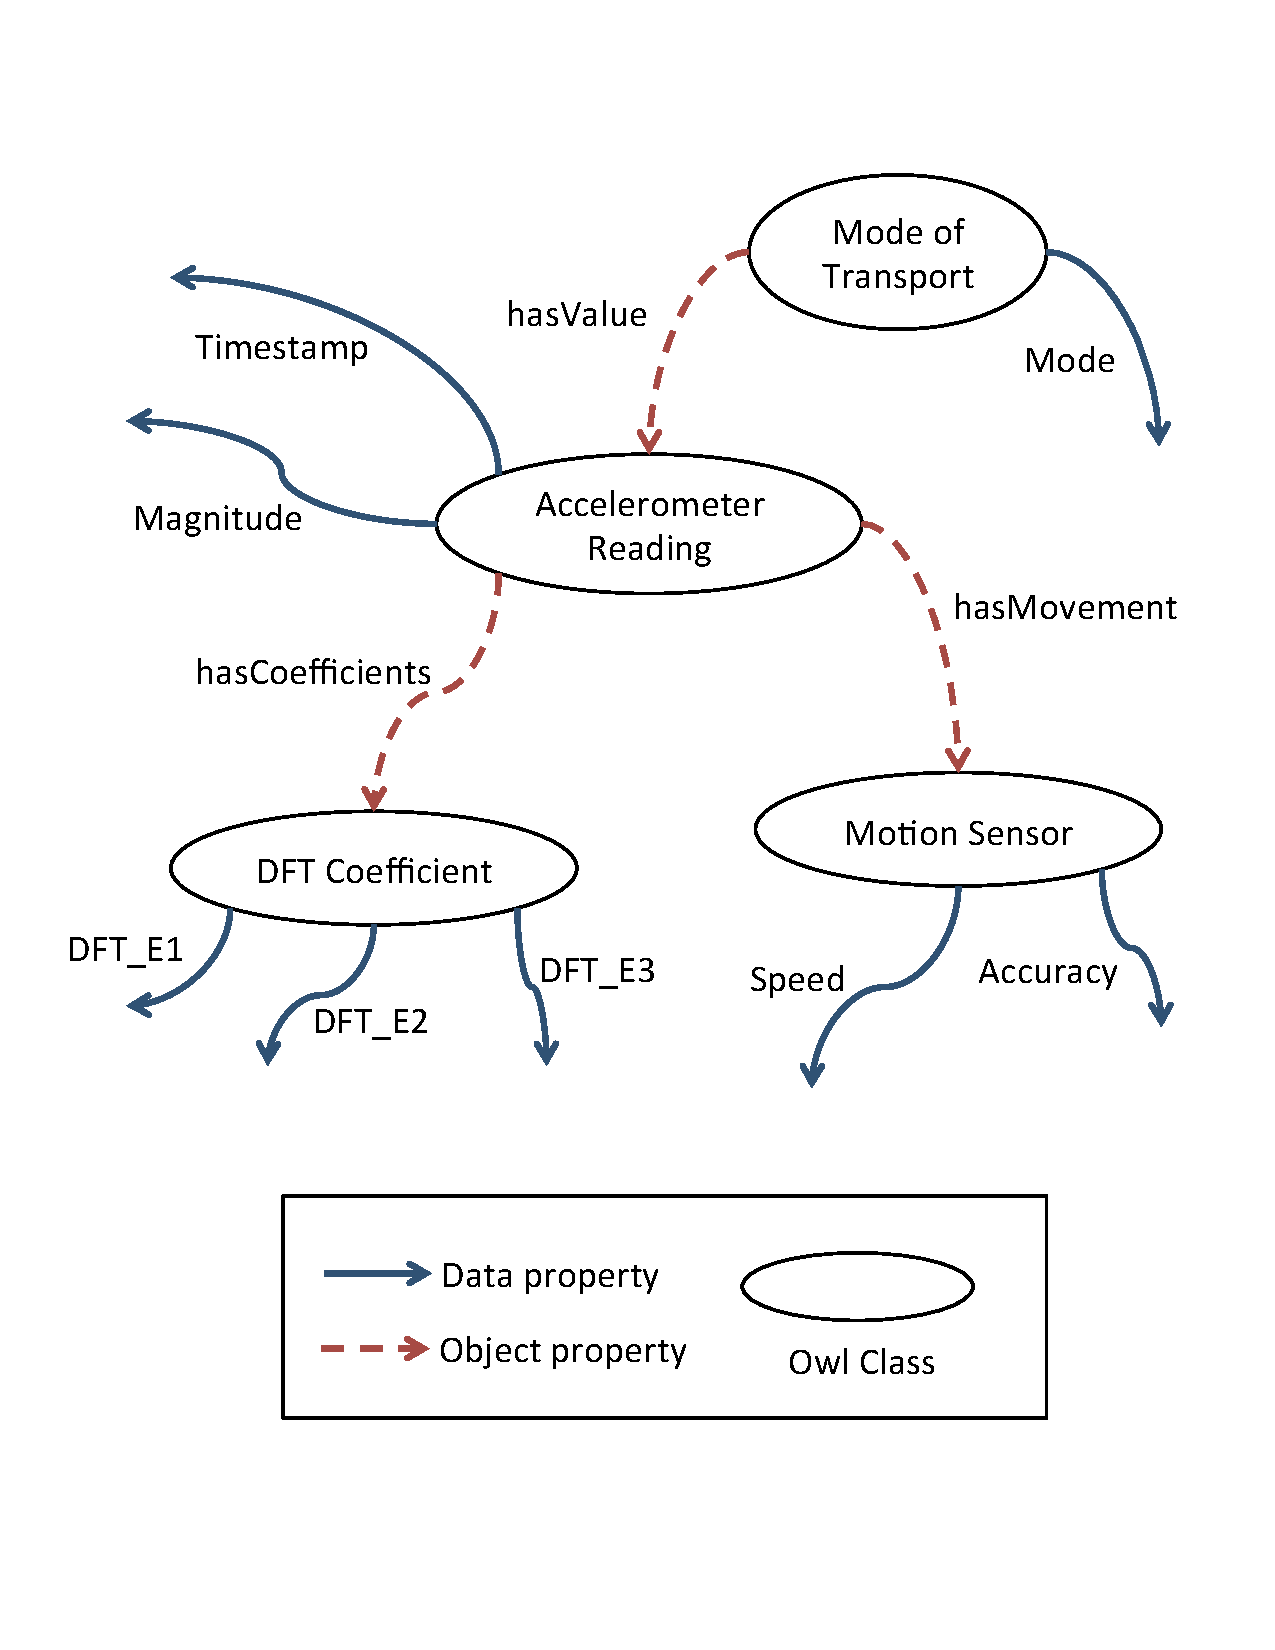
\includegraphics[width=90mm]{img/ontology.pdf}
\caption{Ontology used in for the mode of transportation data\label{fig:ontology}}
\end{figure}

\subsection{Processing with Karma}
The steps using Karma are divided into two parts:
\begin{enumerate}
  \item \textbf{Karma setup}: These are tasks that are performed only the first time. They include modeling the three web services, addDFT, getLabel, and svmTraining, which are explained later, as well as modeling the two raw datasets AccelerometerSensor and LocationProbe. All transformations and processing done here is recorded by Karma and can be played automatically for the other datasets. 
  \item \textbf{Karma execution}: The Karma execution tasks are ones that are repeated for each datasets. They mainly include tasks such as service invocation, joining datasets, and publishing data in the Resource Description Framework (RDF).
\end{enumerate} 

\begin{figure}[bp]
\centering
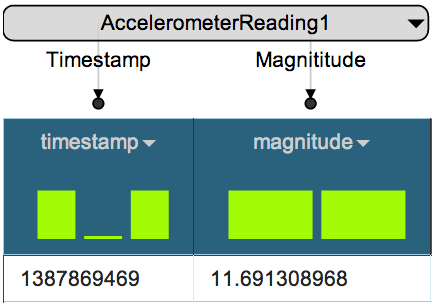
\includegraphics[width=55mm]{img/DFTservice}
\caption{Semantic model for addDFT service\label{fig:dftService}}
\end{figure}

\subsubsection{Karma Setup} 
The work on Karma\cite{knoblock12:eswc} shows how to map structured data to RDF using an ontology. Karma uses a two step process to map data to ontology. The mapping of columns to semantic types and specifying relationships between the semantic types is demonstrated in the work on the Smithsonian dataset\cite{szekely14:ijhac}. When we map our services to our ontology, we attach additional properties to the model along with the semantic type mappings that enables Karma to mark them as a service model. A service model is used to invoke a web service using the columns mapped as inputs to the service. We create an ontology for the mode of transportation data and use it to model our services and data sources. We do not add the ontology creation time in the setup time because such ontologies address a larger domain model and evolve over a period of time. Hence we assume that the ontology was created beforehand. We discuss our ontology and modeling of the services and data sources in the remaining part of the section.

\begin{figure*}[ht!]
\centering
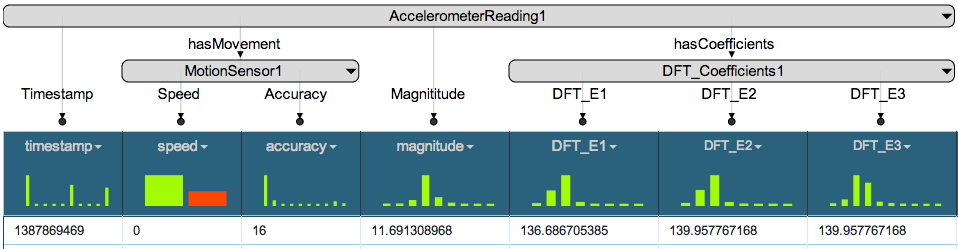
\includegraphics[width=180mm]{img/getLabelService}
\caption{Semantic model for getLabel service\label{fig:imgGetLabelService}}
\end{figure*}

\begin{figure*}[bp]
\centering
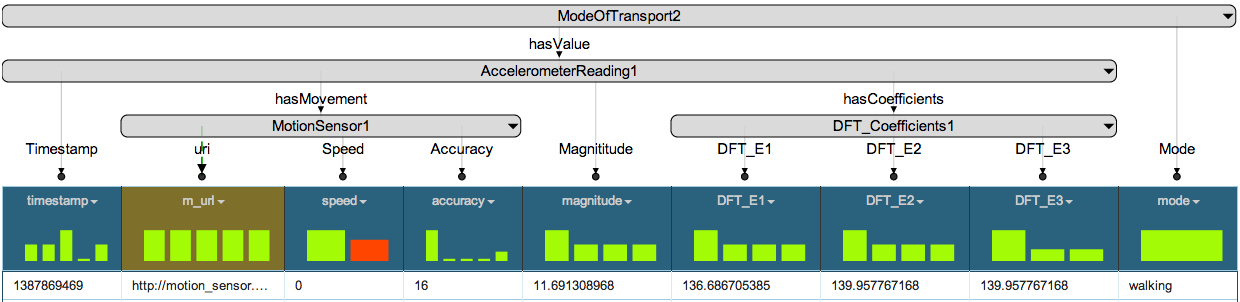
\includegraphics[width=180mm]{img/svmService}
\caption{Semantic model of SVM --- training and testing services\label{fig:svmService}}
\end{figure*}

Figure \ref{fig:ontology} shows the mode of transportation ontology. It contains 4 classes:
\begin{enumerate}
  \item \textit{ModeOfTransport}: Contains a data property for the mode of transportation label
  \item \textit{AccelerometerReading}: Contains data properties for timestamp and acceleration magnitude. The object property --- `hasMovement' connects it to MotionSensor. Similarity, `hasCoefficient' object property connects the AccelerometerReading class to DFT\_Coefficient
  \item \textit{MotionSensor}: Contains data properties for speed and accuracy components of the location probe data
  \item \textit{DFT\_Coefficient}: Contains data properties for the DFT energy coefficients at 1Hz, 2Hz and 3Hz
\end{enumerate} 

We will model three services that we require in our prediction task. Figures \ref{fig:dftService}, \ref{fig:imgGetLabelService} and \ref{fig:svmService} show the models for these services.

The `addDFT' service is a Hypertext Transfer Protocol (HTTP) POST service that calculates the DFT energy coefficients for acceleration magnitude at 1Hz, 2Hz and 3Hz. The input to this service is a CSV file that contains two columns --- timestamp and acceleration magnitude. The DFT values are calculated over a time window of one second. The output generated is a CSV file having the columns --- timestamp, magnitude and the DFT energy coefficients. To model this service, we map the timestamp and magnitude column of our sample CSV file to the appropriate classes. As shown in Figure \ref{fig:dftService}, we set the semantic type of the timestamp column to `timestamp', which is a property of the `AccelerometerReading' class. We then map the magnitude column using the `Magnitude' property of the `AccelerometerReading' class. We set the service URL for the addDFT service and publish the model.

The `getLabel' service is a HTTP POST service that adds the mode of transportation label provided by the user for each row in the input file, using the timestamp values. The output produced is a CSV file containing all the columns of the input with an additional column for labels. To model this service, we map all the columns of our sample CSV file to the appropriate classes excluding the mode column. Figure \ref{fig:imgGetLabelService} shows the column mappings and relationships between the classes, displayed on the Karma interface. We map the speed and accuracy columns to the MotionSensor class using the respective data properties. The timestamp and magnitude are mapped to the AccelerometerReading class. After setting all the semantic types, we set the service URL and other options that are required while invoking the service and publish the model. 

The SVM service has two parts --- training and testing. Both  services take the same set of inputs and have identical semantic types for their corresponding columns. Figure \ref{fig:svmService} shows the semantic model for the SVM training and testing services. The model is very similar to the getLabel service shown in  Figure \ref{fig:imgGetLabelService}. For the SVM service, we map the `mode' column that contains the mode of transportation labels to the `ModeOfTransport' class. The rest of the mappings are discussed in the previous paragraph. We use different service URLs when we publish the SVM training and testing service models. These services also differ in the output that they produce. The training service returns a summary of the SVM model that was trained. In order to distinguish our prediction models, we specify a unique tag in the URL when we train the model. This tag serves as an identifier when we test the model. The testing service produces the prediction output along with the confusion matrix. The output for both the training and testing service is in JSON format. They both consume CSV data in the POST payload.

\begin{figure*}[ht!]
\centering
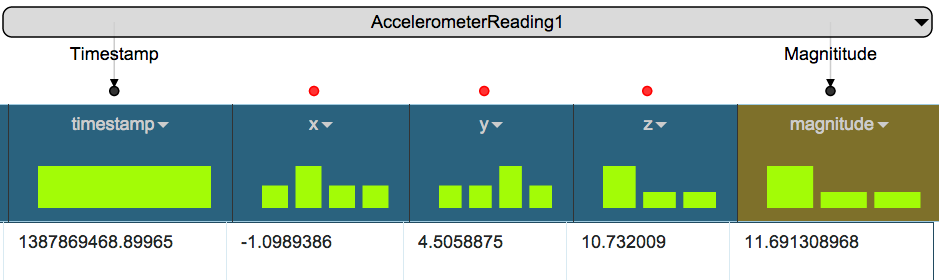
\includegraphics[width=117mm]{img/AccelerometerReadingModel}
\caption{Semantic model for the AccelerometerSensor dataset.\label{fig:AccelerometerReadingModel}}
\end{figure*}

\begin{figure*}[b]
\centering
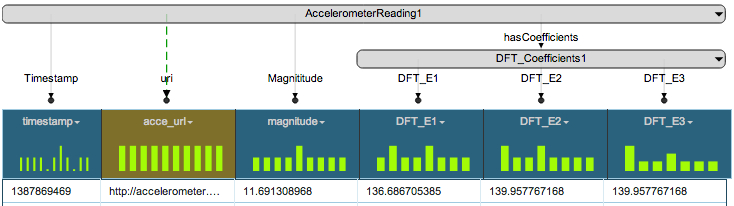
\includegraphics[width=177mm]{img/DFToutput}
\caption{Semantic model of the output generated by addDFT service. \label{fig:DFToutput}}
\end{figure*}

After modeling the services, we model our data sources because the raw data needs to be cleaned and transformed before it can be fed to our services. Karma records the transformations that we perform while modeling the data and replays it when we apply the model on a new file from our data set. After modeling the data, we publish the resulting RDF. Figures \ref{fig:AccelerometerReadingModel}, \ref{fig:DFToutput}, and \ref{fig:motionSensorModel} show the models for our data sources.

Starting with the AccelerometerSensor file, we add the magnitude column using a Python transformation, which is available as a feature in Karma. In this transformation, we calculate the magnitude values using acceleration along x, y, and z coordinates available in the raw data, and by using standard library functions in Python. Figure \ref{fig:AccelerometerReadingModel} shows the resulting model in Karma. The magnitude column appears in yellow color because it is added using a Python transformation and indicates that it is not a part of the original file that is uploaded in Karma. After mapping the semantic types and generating URLs for the classes, we publish the model.

The next data source we model is the output of the addDFT service which is shown in Figure \ref{fig:DFToutput}. The output is a CSV file with the columns --- timestamp, magnitude and DFT energy coefficient values at 1Hz, 2Hz and 3Hz. The addDFT service appends three columns to the input file having headers --- `DFT\_E1', `DFT\_E2' and `DFT\_E3', as shown in Figure \ref{fig:DFToutput}. We map the three columns containing the DFT energy coefficients to the `DFT\_Coefficient' class. The timestamp and magnitude columns are mapped to the `AccelerometerReading' class. We add an additional column, `acce\_url', using a Python transformation and populate it by appending the timestamp values to a base Uniform Resource Identifier (URI). The `acce\_url' column is mapped as the URI for the `AccelerometerReading' class. It is not necessary to have URIs for every class in the model. We add the URI for `AccelerometerReading' class because it is required by Karma to perform join operations.

\begin{figure*}[ht!]
\centering
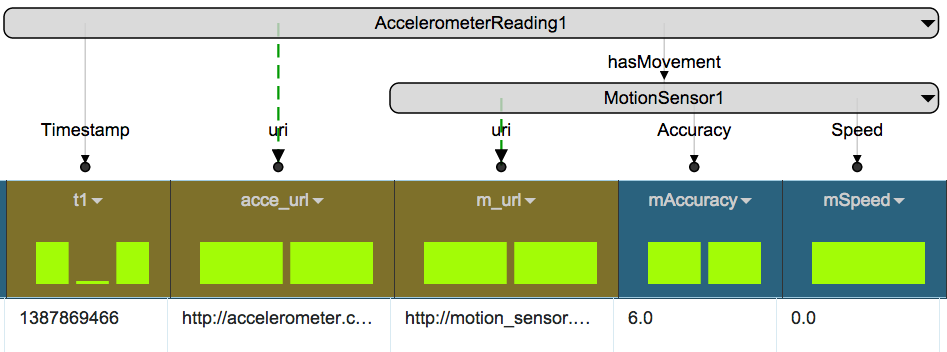
\includegraphics[width=130mm]{img/motionSensorModel}
\caption{Semantic model for the Location probe dataset}
\label{fig:motionSensorModel}
\end{figure*}

The LocationProbe file contains 47 columns, some of them are --- \textit{id, device, timestamp, mAccuracy, mAltitude, mBearing, mElapsedRealtimeNanos, mExtras\_networkLocationSource, mExtras\_networkLocationType, mExtras\_travelState, mHasAccuracy, mHasAltitude, mHasBearing, mHasSpeed, mLatitude, mLongitude, mProvider, mSpeed, mTime, timestamp, etc}. Out of these we only use `timestamp', `mSpeed' and `mAccuracy'. To model this data source, we hide all the unwanted columns after loading the CSV file. As shown in Figure \ref{fig:motionSensorModel}, we map the accuracy and speed columns to the `MotionSensor' class and the timestamp to `AccelerometerReading' class. We generate two additional columns --- `acce\_url' and `m\_url' to add URIs for the `AccelerometerReading' and `MotionSensor' classes. The URIs are generated using a Python transformation, by appending the timestamp value to a base URI. This completes the Karma setup process.

\subsubsection{Karma Execution} 
Once we have modeled all our data sources and services, we start with the Karma execution steps to process the mode of transportation data. Our goal is to integrate all the datasets to produce a CSV file that can be fed to the SVM algorithm. In Karma, we do this by first modeling each dataset according to the ontology, then publishing the data as RDF, and finally using join operations to merge the data.

\begin{figure*}[bp]
\centering
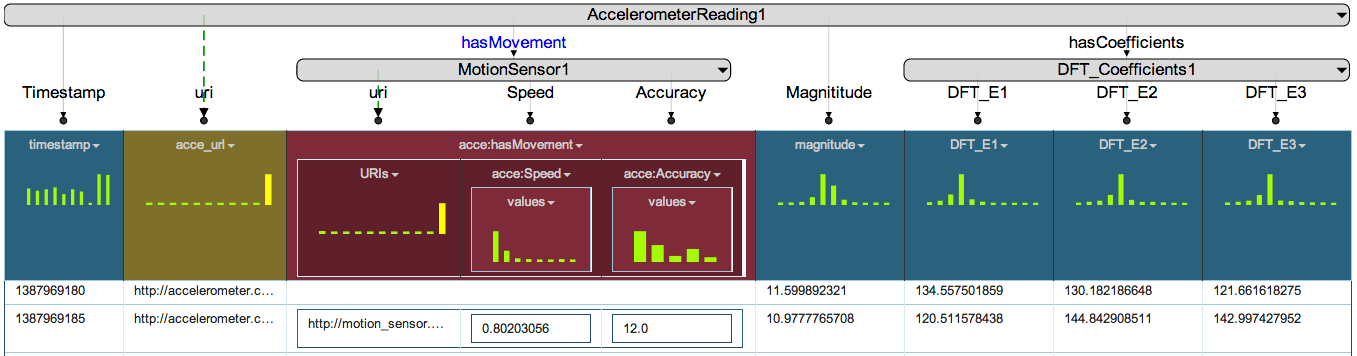
\includegraphics[width=184mm]{img/model_after_augmentation}
\caption{Karma worksheet after joining the accelerometer and location datasets}
\label{fig:model_after_augmentation}
\end{figure*}

We load the LocationProbe file, apply the `LocationProbe' model, and publish the resulting RDF. For the accelerometer sensor data, we start by loading the data collected for the first day. We apply the `AccelerometerSensorModel' and publish the RDF. To invoke the addDFT service, we select the `Invoke Service' option from the drop down menu that appears after clicking the AccelerometerReading class bubble. Karma distinguishes between service models and data models and shows the list of services that could be invoked. Karma determines that a service can be invoked if the semantic type mappings for all the input columns along with the relationships between the classes match with the model on the current worksheet. From the list of services shown, we select the addDFT service and then select the corresponding RDF graph where the accelerometer data was published. The results of the addDFT service are loaded in a new worksheet. We apply the model that was created for the addDFT output to the new worksheet and publish RDF. After we have published the data from the addDFT service, we perform a join operation with the LocationProbe data that was published previously. Starting from the topmost class in the model, i.e., AccelerometerReading, we use the `Augment Data' option to perform the join.

Karma explores the properties that could be added to the selected class, in this case the AccelerometerReading class, which are not currently present in the worksheet. Karma fetches the additional properties from the available RDF data in the triple store. In our ontology, the AccelerometerReading class has an object property `hasMovement' that connects it to the MotionSensor class. We select this property to be added in the worksheet. Karma adds a URL column for the MotionSensor class and populates it with the joined values. We repeat the join process for the MotionSensor class and add the speed and accuracy properties. The final augmented worksheet is shown in Figure \ref{fig:model_after_augmentation}. The yellow colored columns are added through transformations and the red columns are the ones that get attached by joining the location probe data. The columns in blue are part of the original model. We then publish the augmented model and the RDF in a new graph. We need to publish this model because the model shown in Figure \ref{fig:model_after_augmentation} is not the original model and contains additional properties that were added after the join operation. 

We now invoke the getLabel service to add the mode of transport column. The service creates a new worksheet to which we apply the SVM model as shown in Figure \ref{fig:svmService}, and publish the RDF. Since this is the first file that we process, we will invoke the SVM training service and use the processed data as training set. For the succeeding files, we first invoke SVM testing service and evaluate our model for the accuracy. Then we publish RDF for the test dataset to append it to the same graph that we used in the previous iteration. We use the merged data as a training set and again train our SVM model by invoking the SVM training service. We do this iteratively for the data for all the days that follow. Thus, as we process more data files, and add to the training set, our model improves in the prediction accuracy. The JSON results of the service invocation are parsed and loaded in a new worksheet. 